\section{Home Activity}
This section will explain what the \activity{Home Activity} provides of services to the user.\\\\

This activity is the center of the launcher and implements the design described in \autoref{design:app_manangement}. As the center it also have a lot of functionality some of it is the drawer which is explained in \autoref{GUI:drawer}. 
Some of the more basic functionality is to show the user which apps they can open. This is done by showing all apps which is installed on the device, is certified as an app in the database and the user has a relation to the apps in the database. Only apps which has all of these three properties will be shown to the user. If this number of apps exceeds nine and or if the drawer is extended so much that some apps will be place to the right of the screen the user will be able to scroll horizontally and will be guided by a scroll indication bar in the bottom of the screen.

\subsection{The drawer}
The drawer mentioned in \autoref{sec:drawer} was also implemented.

The drawer is a place for functionality, this could be e.g. a way to put apps in the drawer if they are not being used by the user or if they need them they can drag them out of the drawer \autoref{backlog:hide_apps}.

\begin{figure}[h!]
	\centering
	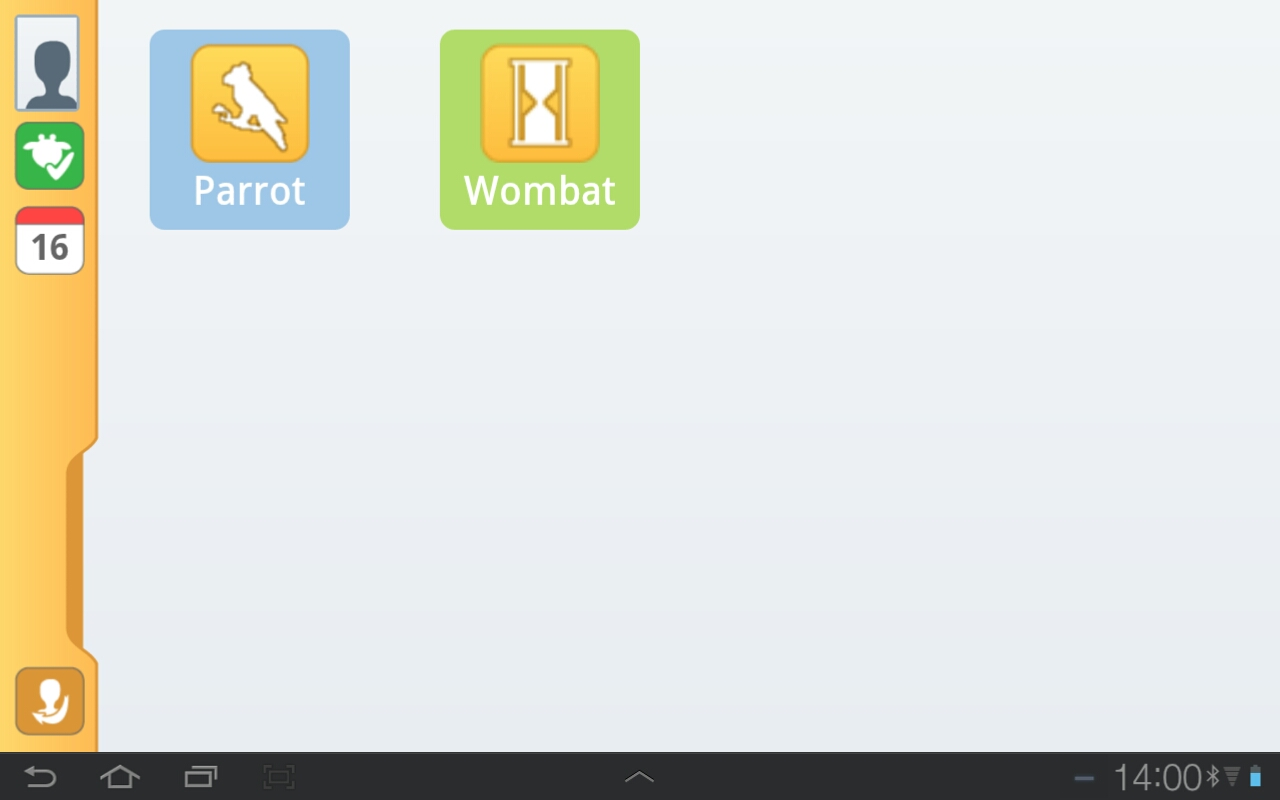
\includegraphics[scale=0.2]{gfx/home-activity_closed}
	\caption{Shows the launcher with the drawer closed.}
	\label{fig:home-activity_closed}
\end{figure}

\begin{figure}[h!]
	\centering
	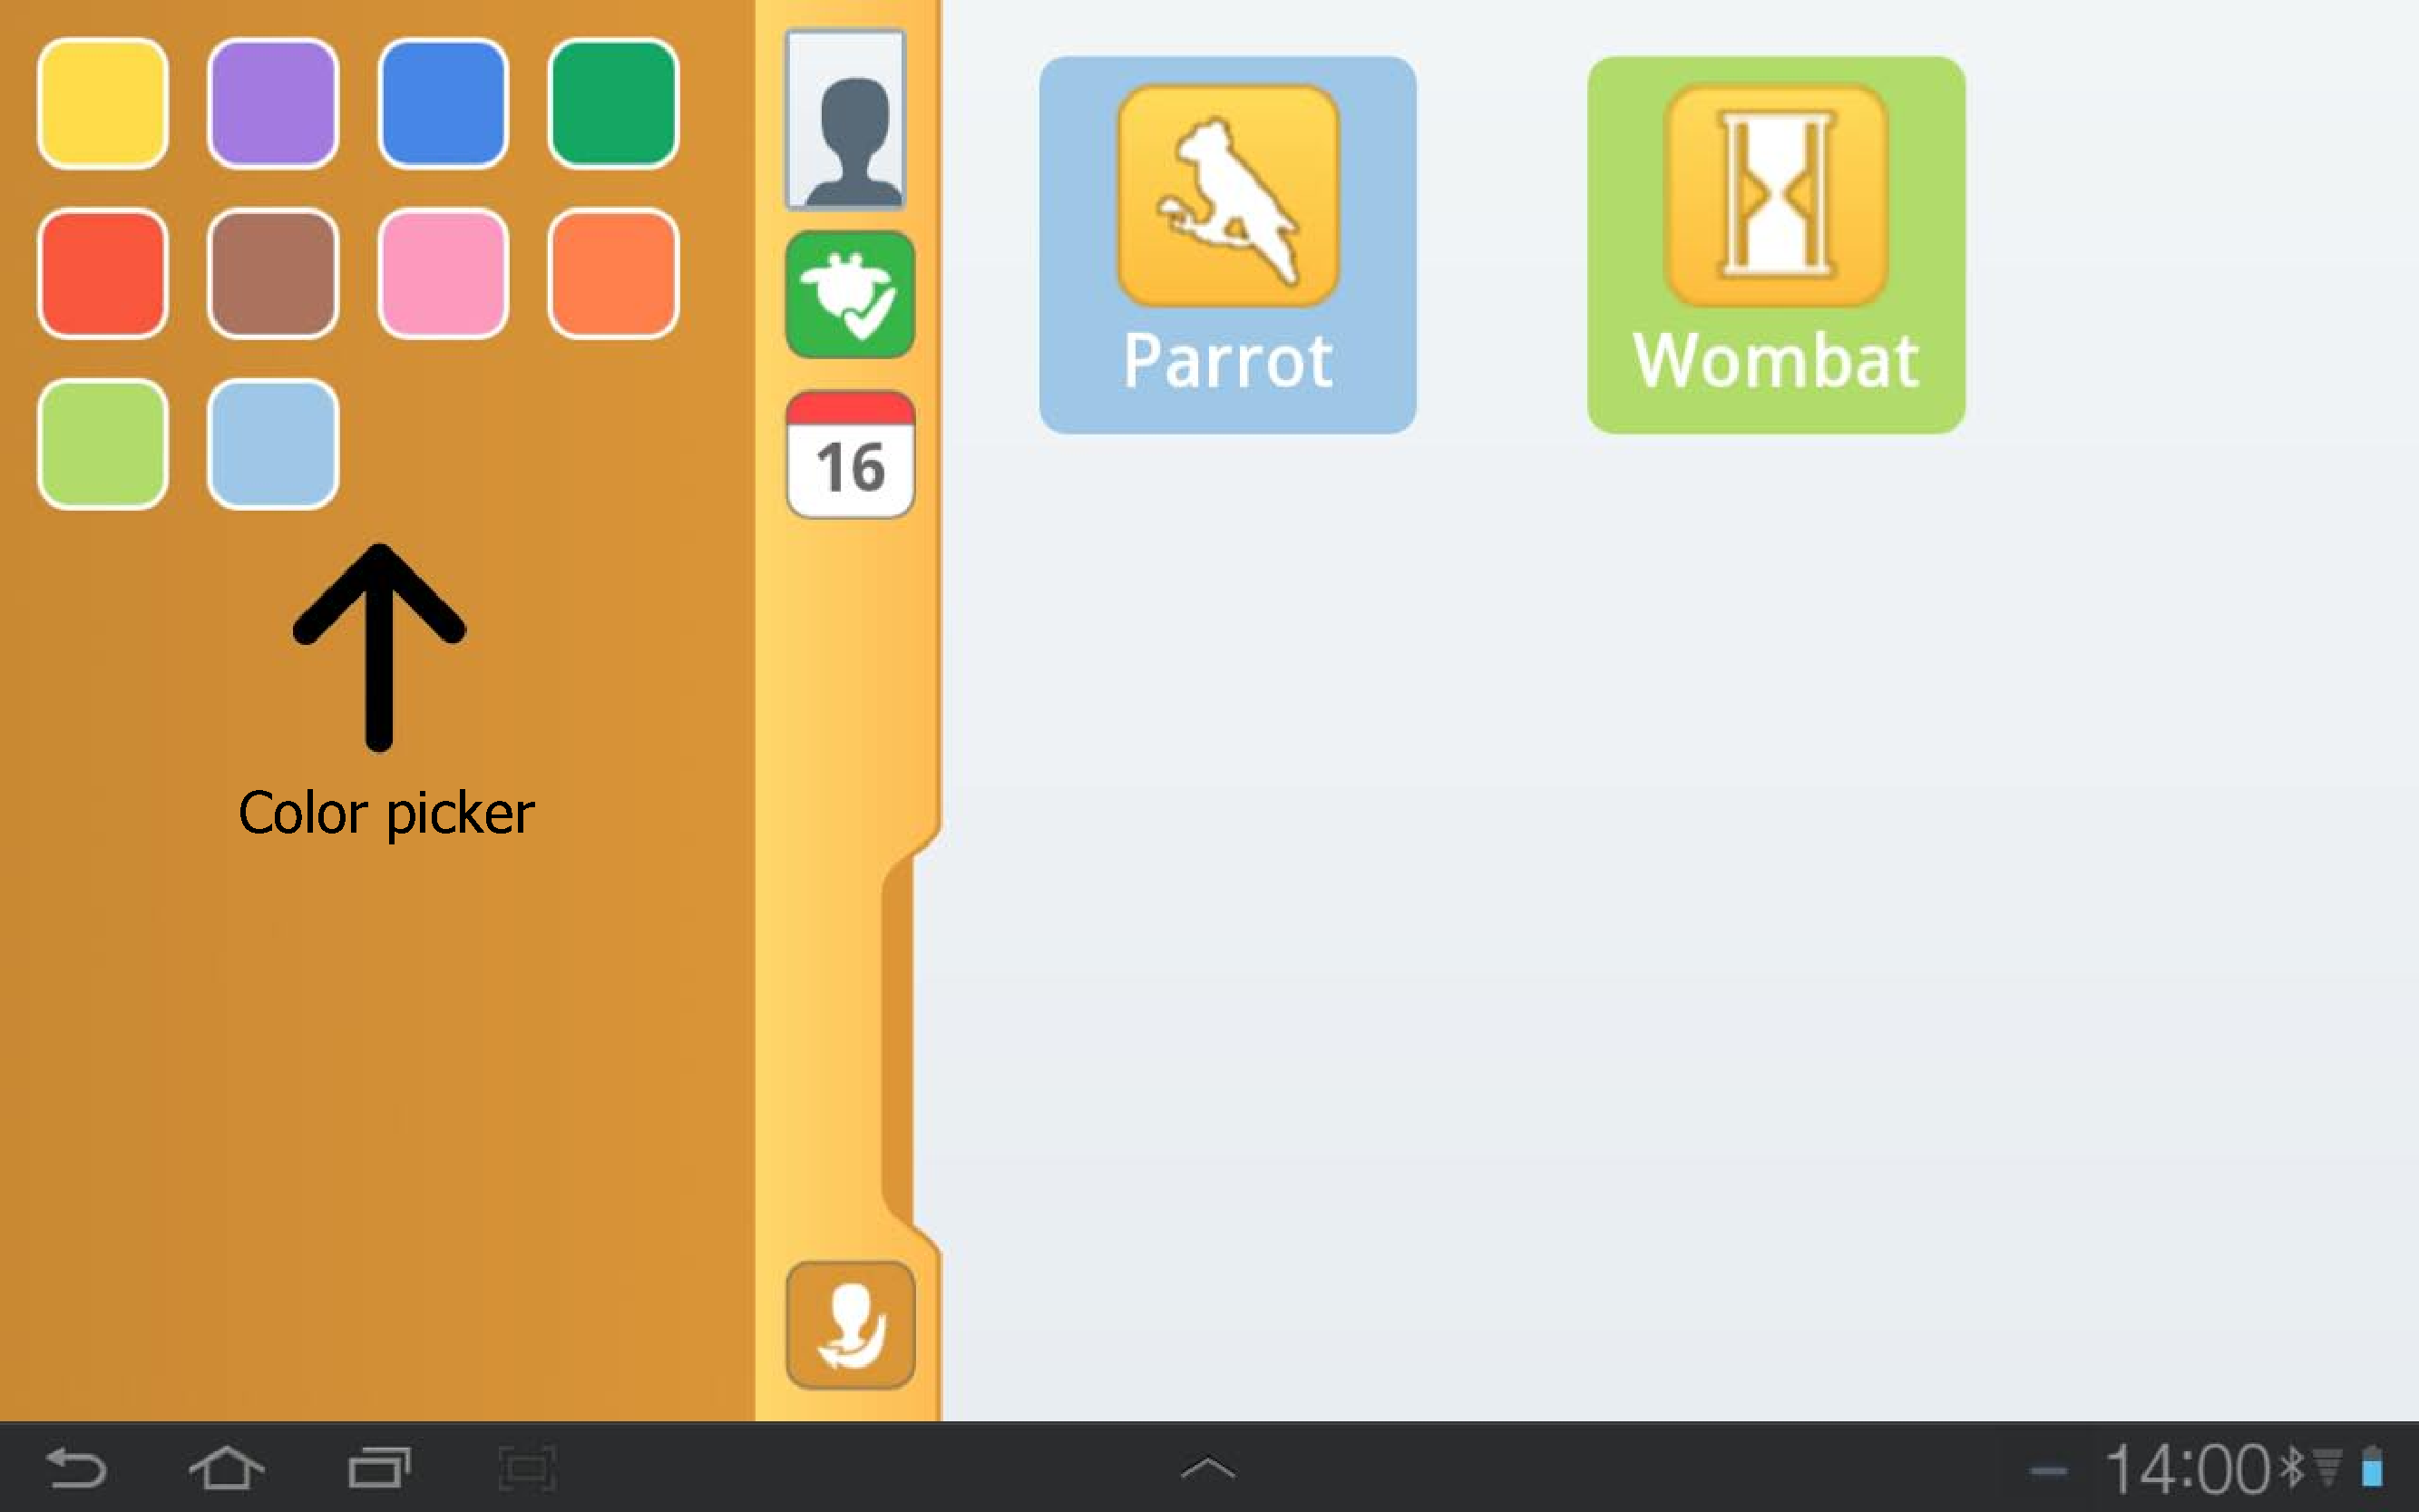
\includegraphics[scale=0.2]{gfx/home-activity_open}
	\caption{Shows the launcher with the drawer opened. The color picker can also be seen here.}
	\label{fig:home-activity}
\end{figure}

\subsection{Color picker}
\label{home:colorpicker}

To show the functionality of the drawer a color picker for apps were implemented and hidden in the drawer. The color picker can be seen in \autoref{fig:home-activity} as mentioned in \autoref{backlog:homebar_drawer} and explained in \autoref{design:app_manangement}.
The \textit{color picker} is a tool that was made to change colors on apps, this have been extended so far that if the logo of e.g. WOMBAT is choosen to be red then the background in WOMBAT will also be set to red when the application is loaded.

The color picker is implemented with a color board with ten predefined \giraf[] colors. These colors can be assigned to any app that are in the launcher and there is no limit on how many times the user can use one color. This means that if the user want they can make every app e.g. red.
The color picker is made with drag and drop functionality as described in \autoref{par:colorpicker}. When the user have choosen a color and assigned it the app icon will change to this color and the color is saved in the local database so that if the user restarts the launcher the apps will still have the colors the users have assigned for them. 
The color picker can be seen in \autoref{fig:home-activity}

\subsection{Widgets}

The widgets which is described in \autoref{par:widgets} and can be seen in \autoref{fig:home-activity}is between the app board and the drawer, this is called the \textit{home bar}. Here it is also possible to see a picture of the user curretly logged in. The user can logout with the orange button in the button of the home bar. There are two widgets: One that shows the connectivity to the Savanah server. This widget has three states: Connected and updated, connected and synchronising and not connected. Connected and updated tells the user that all data is synchronized with the server and they are good to go. Connected and synchronising means that either the tablet needs data from the server or to push some changes to the server. Not connected tells the user that they are not connected to the server and therefore can not update or synchronize with the server.
If the user clicks on the connectivity widget they will get a description to the currently showing status telling them what this icon means.
The second widget is a calendar widget which tells the user what day it is in the month in a numeric format. If the user clicks this widget they will get a description with day, d. dd, month, week. This is done so the user easily can access and see what day it is.


\begin{lstlisting}[style=sourceCode, language=JAVA, caption=This is code, label=lst:homeActivity] 
\end{lstlisting}